\section{Middleware}

Middleware is a software layer between software applications and operating systems that provide services to the applications apart from the ones available from the operating systems \parencite{Bernstein:1996:MMD:230798.230809}. For software developers to focus on the specific purpose of the application, middleware makes implementation of input/output and communication easier.

In the context of distributed systems, middleware is responsible for communication and management of data among the nodes. It simplifies various systems that support application development and delivery like web servers, messaging systems, application servers and other similar systems. The primary purpose of a middleware system is to provide the abstraction for the complex interaction that takes between heterogeneous nodes in a distributed system. The complexity of services such as concurrency, location, naming and service discovery are hidden from the application layer. It does so by providing a common Application Programming  Interface. Figure \ref{figures:middleware} depicts a typical high-level design of the involvement of middleware in a distributed systems scenario.

\makeatletter
\setlength{\@fptop}{0pt}
\makeatother

\begin{figure}[t!]
\centering
\def\svgwidth{.8\textwidth}
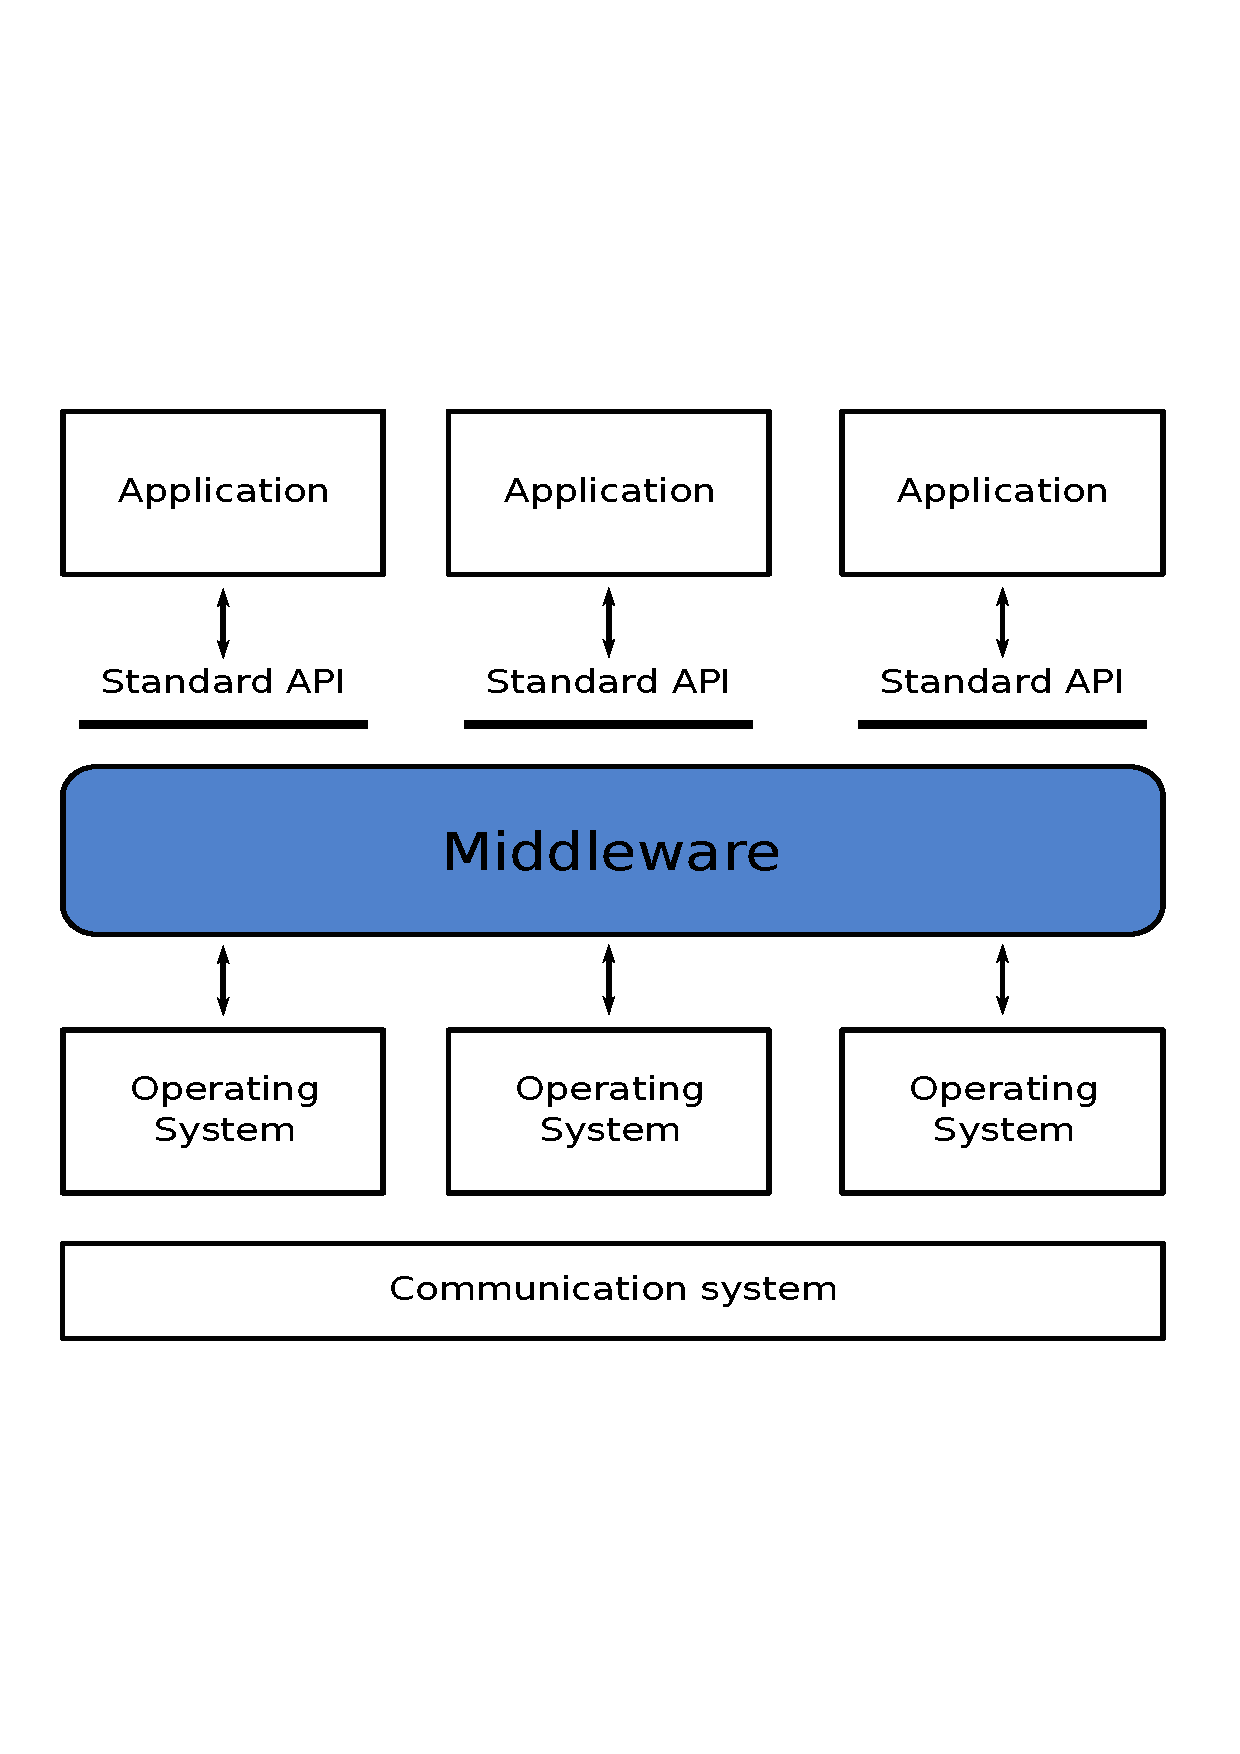
\includegraphics[keepaspectratio, width=.6\textwidth, trim={0 7cm 0 6cm},clip]{middleware.pdf}
\caption{Middleware}\label{figures:middleware}
\end{figure}

There are many types of middleware \parencite{middleware_types}. Few of them are listed below:

\begin{itemize}
  \item \textbf{Message Oriented Middleware:} These are the class of middleware systems that perform routing and transformation of messages. These are asynchronous in their nature of operation. A good example is integration brokers. 

  \item \textbf{Remote Procedure Call (RPC) Middleware:} As the name suggests these class of middleware is used to calling procedures on remote systems. The interaction between the caller and callee systems can be synchronous or asynchronous.

  \item \textbf{Database Middleware:} These middleware allows direct interaction with databases. Extract, Transform, and Load (ETL) tools like Pentaho come under this category

  \item \textbf{Embedded Middleware:} These type of middleware allows embedded applications to communicate with real-time operating systems.

  \item \textbf{Portals:} These middleware deal with the interaction between the front end and the back end services.
\end{itemize}